\section{WS 1.1 - 9 Verurteilungen Jugendliche - MC - Matura
2015/16 - Nebentermin 1}

\begin{beispiel}[WS 1.1]{1} %PUNKTE DES BEISPIELS
	
Jugendliche sind laut Jugendschutzgesetz 1988 (Fassung vom 23.3.2016) Personen, die das
14.�Lebensjahr, aber noch nicht das 18. Lebensjahr vollendet haben. Die nachstehende Grafik
zeigt f�r den Zeitraum von 1950 bis 2010 sowohl die absolute Anzahl der Verurteilungen Jugendlicher
als auch die Anzahl der Verurteilungen Jugendlicher bezogen auf 100000 Jugendliche. \leer

				
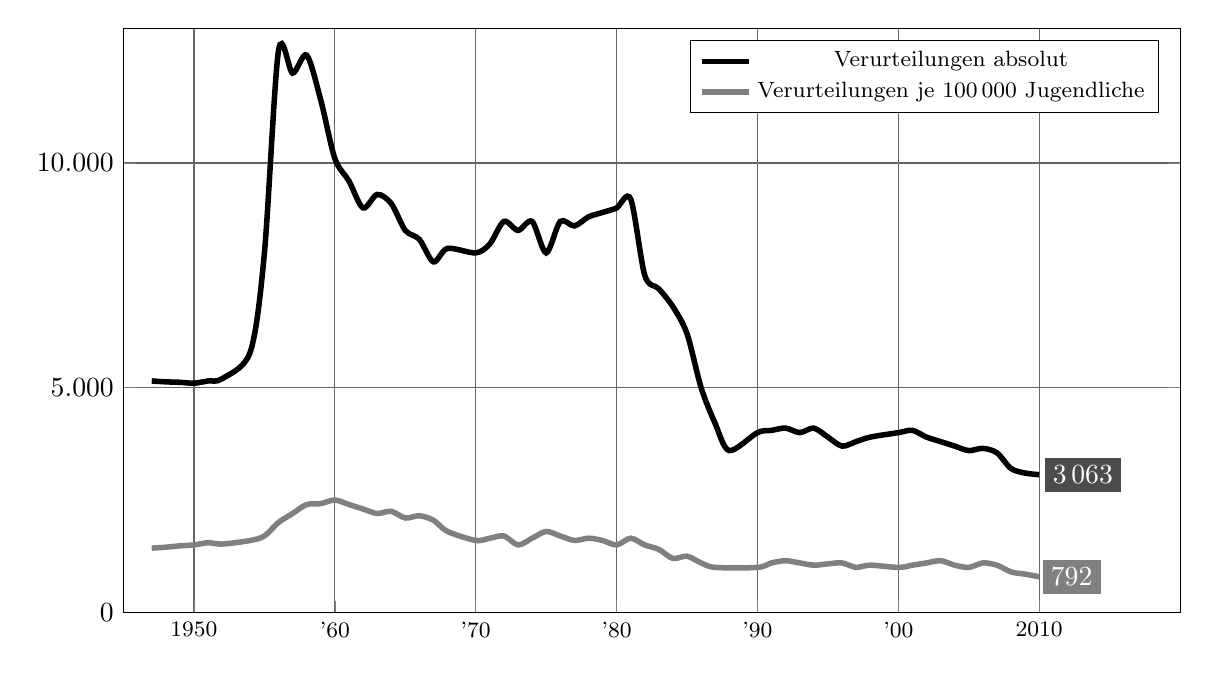
\begin{tikzpicture}
\begin{axis}
[xmin=-0.5,xmax=7,height=9cm, width=15cm,scaled ticks = false,xtick={0,1,...,7}, xtick pos=left,
xticklabels={1950,'60, '70, '80, '90, '00, 2010}, xticklabel style={font=\footnotesize,
minor x tick num={0}, align=center},
xmajorgrids,
ymajorgrids,
ytick={0,5000,10000},
yticklabels={0,5.000,10.000},
ymin=0,
ymax=13000,
grid style={black!60}
]

\addplot[smooth,
    color=black,
    mark=,
		line width=2pt,
    ]
    coordinates {
		(-0.3,5150)(-.2,5130)(-.1,5120)		(0,5100)		(0.1,5150)  (0.2,5200) (0.4,5800)	(0.5,8000)	(0.6,12500)	(0.7,12000)	(0.8,12400)	(0.9,11400)	(1.0,10100)	(1.1,9600)	(1.2,9000)	(1.3,9300)	(1.4,9100)	(1.5,8500)	(1.6,8300)	(1.7,7800)	(1.8,8100)	(2,8000)	(2.1,8200)	(2.2,8700)	(2.3,8500)	(2.4,8700)	(2.5,8000)	(2.6,8700)	(2.7,8600)	(2.8,8800)	(2.9,8900)	(3,9000)	(3.1,9200)	(3.2,7500)	(3.3,7200)	(3.4,6800)	(3.5,6200)	(3.6,5000)	(3.7,4200)	(3.8,3600)	(4,4000)
		(4.1,4050)	(4.2,4100)	(4.3,4000)	(4.4,4100)	(4.5,3900)	(4.6,3700)	(4.7,3800)	(4.8,3900)	(5,4000)	(5.1,4050)	(5.2,3900)	(5.3,3800)	(5.4,3700)	(5.5,3600)	(5.6,3650)	(5.7,3550)	(5.8,3200)	(5.9,3100) (6,3063)		
    };
\addlegendentry{\footnotesize Verurteilungen absolut}
\addplot[smooth,
    color=black!50,
    mark=,
		line width=2pt,
    ]
    coordinates {(-0.3,1430)	(-.2,1450)	(-.1,1480)	(0,1500)	(0.1,1550)   (0.2,1520)	(0.4,1600)	(0.5,1700)	(0.6,2000)	(0.7,2200)	(0.8,2400)	(0.9,2420)	(1.0,2500)	(1.1,2400)	(1.2,2300)	(1.3,2200)	(1.4,2250)	(1.5,2100)	(1.6,2150)	(1.7,2050)	(1.8,1800)	(2,1600)	(2.1,1650)	(2.2,1700)	(2.3,1500)	(2.4,1650)	(2.5,1800)	(2.6,1700)	(2.7,1600)	(2.8,1650)	(2.9,1600)	(3,1500)	(3.1,1650)	(3.2,1500)	(3.3,1400)	(3.4,1200)	(3.5,1250)	(3.6,1100)	(3.7,1000)	(3.830)	(4,1000)	(4.1,1100)	(4.2,1150)	(4.3,1100)	(4.4,1050)	(4.5,1080)	(4.6,1100)	(4.7,1000)	(4.8,1050)	(5,1000)	(5.1,1050)	(5.2,1100)	(5.3,1150)	(5.4,1050)	(5.5,1000)	(5.6,1100)	(5.7,1050)	(5.8,900)	(5.9,850)	(6,792)		
    };
\addlegendentry{\footnotesize Verurteilungen je 100\,000 Jugendliche}

%\draw(200,10) node[]{\colorbox{black!70}{\textcolor[rgb]{1,1,1}{3\,063}}};
%%\draw(674,8) node[]{\colorbox{black!50}{\textcolor[rgb]{1,1,1}{792}}};
%rtt

\pgfplotsset{
    after end axis/.code={
        \node[] at (axis cs:6.31,3063){\colorbox{black!70}{\textcolor[rgb]{1,1,1}{3\,063}}};
				\node[] at (axis cs:6.23,792){\colorbox{black!50}{\textcolor[rgb]{1,1,1}{792}}};
    }
}
\end{axis}
\end{tikzpicture}


\leer

Wie viele Jugendliche insgesamt gab es in �sterreich in etwa im Jahr 2010?
Kreuze die zutreffende Anzahl an.

\multiplechoice[6]{  %Anzahl der Antwortmoeglichkeiten, Standard: 5
				L1={792\,000},   %1. Antwortmoeglichkeit 
				L2={3\,0630\,000},   %2. Antwortmoeglichkeit
				L3={3\,863\,000},   %3. Antwortmoeglichkeit
				L4={387\,000},   %4. Antwortmoeglichkeit
				L5={258\,000},	 %5. Antwortmoeglichkeit
				L6={2\,580\,000},	 %6. Antwortmoeglichkeit
				L7={},	 %7. Antwortmoeglichkeit
				L8={},	 %8. Antwortmoeglichkeit
				L9={},	 %9. Antwortmoeglichkeit
				%% LOESUNG: %%
				A1=4,  % 1. Antwort
				A2=0,	 % 2. Antwort
				A3=0,  % 3. Antwort
				A4=0,  % 4. Antwort
				A5=0,  % 5. Antwort
				}

			
\end{beispiel}